\clearpage
{\bfseries SRSTI 52.13.05}

\section{THE INFLUENCE OF TECHNOGENIC FACTORS ON THE EFFECTIVE COMBINED DEVELOPMENT OF ORE DEPOSITS}

\begin{center}
{\bfseries M.B. Baizbayev\textsuperscript{1*}, S.B.
Aliyev\textsuperscript{2}, A.D. Shontayev\textsuperscript{3}, D.D.
Meiram\textsuperscript{3}, E.K. Karzhauova\textsuperscript{3}}

{\bfseries \textsuperscript{1,3}} Kazakh University of Technology and
Business, Astana, Kazakhstan Institute of Problems

of Complex Development of Subsoil named after academic N.V.Melnikov
(IPKON RAN), Moscow, Russian Federation,

e-mail: \href{mailto:baiz76@mail.ru}{\nolinkurl{baiz76@mail.ru}}
\end{center}

The predominant field of application of the complex open-underground
method is extended steep-falling deposits with a homogeneous nature of
mineralization. The main factors influencing the choice of a specific
technological scheme are the capacity of the deposit, the value of the
ore and the stability of the array. The complexity of solving
geomechanical problems determines the main factors of choosing an
open-underground technology - the state of the treatment space and the
way to control the state of the array.

{\bfseries Keywords:} combined geotechnology, technogenic space, mountain
range, deformation, geomechanical processes.

\begin{center}
{\large\bfseries РУДАЛЫҚ КЕН ОРЫНДАРЫН ТИІМДІ АРАЛАС ИГЕРУГЕ ТЕХНОГЕНДІК ФАКТОРЛАРДЫҢ ӘСЕРІ}

{\bfseries М.Б Баизбаев\textsuperscript{1*}, С.Б.Алиев\textsuperscript{2},
А.Ж.Шонтаев\textsuperscript{3}, Д.Д.Мейрам\textsuperscript{3}, Э.К.
Қаржауова\textsuperscript{3}}

{\bfseries \textsuperscript{1,3}}Қазақ технология және бизнес университеті,
Астана, Қазақстан

{\bfseries \textsuperscript{2}}Ресей ғылым академиясы акад. Н.В.Мельников
атындағы Жер қойнауын

кешенді игеру мәселелерінің институты (ИПКОН РАН), Мәскеу, Ресей
Федерациясы,

e-mail: \href{mailto:baiz76@mail.ru}{\nolinkurl{baiz76@mail.ru}}
\end{center}

Күрделі ашық жерасты әдісін қолданудың басым саласы біркелкі минералдану
үлгісімен созылған тік шөгінді кен орындары болып табылады. Нақты
технологиялық схеманы таңдауға әсер ететін негізгі факторларға кен
орнының қалыңдығы, кеннің құндылығы және массивтің тұрақтылығы жатады.
Геомеханикалық есептерді шешудің күрделілігі ашық жер асты технологиясын
таңдаудың негізгі факторларын анықтайды - өндіріс аймағының жағдайы және
массивтің күйін басқару әдісі.

{\bfseries Туйін сөздер:} \emph{~}аралас геотехнология, техногендік
кеңістік, тау-кен массиві, деформация, геомеханикалық процестер.

\begin{center}
{\large\bfseries ВЛИЯНИЕ ТЕХНОГЕННЫХ ФАКТОРОВ НА ЭФФЕКТИВНУЮ КОМБИНИРОВАННУЮ РАЗРАБОТКУ РУДНЫХ МЕСТОРОЖДЕНИЙ}

{\bfseries М.Б.Баизбаев\textsuperscript{1*}, С.Б.Алиев\textsuperscript{2},
А.Д.Шонтаев\textsuperscript{3}, Д.Д.Мейрам\textsuperscript{3},
Э.К.Каржауова\textsuperscript{3}}

Казахский университет технологии и бизнеса, Астана, Казахстан,

Институт проблем комплексного освоения недр имени акад. Н.В.Мельникова

Российской академии наук (ИПКОН РАН),

e-mail: \href{mailto:baiz76@mail.ru}{\nolinkurl{baiz76@mail.ru}}
\end{center}

Преимущественная область применения комплексного открыто-подземного
способа - протяженные крутопадающие месторождения с однородным
характером оруденения. Основными факторами, влияющими на выбор
конкретной технологической схемы, являются мощность залежи, ценность
руды и устойчивость массива. Сложность решения геомеханических задач
определяет основные факторы выбора открыто-подземной технологии -
состояние очистного пространства и способ управления состоянием массива.

{\bfseries Ключевые слова:} комбинированная геотехнология, техногенное
пространство, горный массив, деформация, геомеханические процессы.

\begin{multicols}{2}
{\bfseries Introduction.} A characteristic feature of the combined
development is the presence of quarry and underground treatment spaces
located in the immediate vicinity. The combination of open-pit and
underground operations or the transition from open-pit mining to the
underground method highlights the geomechanical aspects of the choice of
technological schemes and development parameters. This is due to the
need for joint assessments of the state of the mountain range near
underground workings and the side-worked sides of the quarry. The
presence of a technogenic space formed by an open mining method
significantly complicates the geomechanical situation in the zone of
underground work, changing the stress-strain state of elements of
underground mining systems, creating zones of concentration and stress
relief. On the other hand, the presence of extensive underground
mined-out spaces leads to the softening and destruction of the rocks of
the overlying massif, reducing the stability of the sides of the
quarries, supporting and dividing pillars. Forecasting the behavior of
the rock massifs being worked on, assessing the stability of outcrops,
determining rational technological parameters of development in this
case can be based only on the study of geomechanical processes occurring
in the zone of mutual influence of underground and open-pit works.
Prerequisites for the successful solution of the problems of combined
development, ensuring its effectiveness is achieved by knowing the
patterns of distribution of stresses, deformations, displacements formed
in the array during the operation of the field in a combined way.
Research in these areas is a methodological basis for substantiating the
parameters of combined technologies, such as rational opening and
preparation schemes, reliable methods for managing the state of the
arrays being worked on {[}1{]}.

Carrying out underground mining operations in the zone of influence of
the quarry (under the bottom and in the sides) causes a redistribution
of stresses in the developed array. The change in the stress state of
the rock mass causes, in turn, the redistribution of values and the
direction of action of the shifting and holding forces.

The degree of softening of rocks as a result of mining can be different
and depends on the specific conditions of the deposit: the intensity of
structural fragmentation of the massif; orientation of the weakening
planes relative to underground treatment workings and quarry elements;
the initial strength of the massif; the stage of development of the zone
of displacement of the degree of mining of the massif; the speed of
mining, etc {[}2{]}.

The influence of the technogenic space formed by the quarry on
underground mining operations was also studied in order to determine the
preferred order and direction of mining development in the transition
zone of the deposit. Variants of the direction of development of
underground works from the massif to the slope and from the slope to the
array were investigated. The direction of development of underground
mining vertically does not have a significant impact on the formation of
stress fields in the underworked board. In order to intensify the work
and ensure the stability of the sides, on the first underground horizon
at the base of the quarry, it is preferable to develop reserves with
division into panels, continuous excavation of reserves.

The factors determining the use of open-underground technology in the
fields are: the joint use of mine workings for transportation and
drainage; the most complete development of the reserves of the deposit;
the use of waste rocks as a laying material with a simplified scheme of
feeding them into the mine. The factors limiting the use of this method
are disadvantages: the need to reduce the seismic impact of quarry and
underground explosions on the quarry massif; difficult conditions for
ventilation of mine workings.

{\bfseries Materials and methods.} The open-underground mining of deposits
is characterized by a number of features that determine the conditions
of mining operations {[}3{]}.

First, under the influence of underground work, rock movements and
subsidence of the surface are likely. One of the conditions for choosing
underground mining systems during joint work is the need for permanent
and temporary preservation of the stability of the array. The choice of
the development system depends on the specific mining and geological
conditions and the possibility of providing a reliable guarantee of work
safety.

Secondly, the mutual influence of blasting operations in a quarry and in
an underground mine introduces restrictions and should be taken into
account when drawing up plans, calculating BVR passports.

The third is that the joint technology of conducting underground and
open-pit work requires special organization of labor at quarry ore
outlets underground and at drainage works.

Fourth, the high responsibility and complexity of solving geomechanical
tasks imply: calculation of the parameters of safe berms between open
and underground works; assessment of the thickness of the ceiling over
individual sections of the worked-out space; calculation of the
parameters of the supporting pillars and the strength of the hardening
bookmark; determination of the permissible area of horizontal exposure
of the roof of the cleaning space; assessment of the stability of the
sides of the quarry being worked by underground workings.

Currently, in most methods of assessing the stability of slopes, only
the matching stresses due to the action of gravitational forces are
taken into account, and the maximum height of the slope is found by
solving the equation of equilibrium of holding and shifting forces along
the selected sliding surface in the vertical plane. The value of the
stability coefficient of the side depends on the presence of natural
tectonic forces in the rock mass, the ratio of the elastic
characteristics of the rocks composing the mountain range, the ratio of
the geometric dimensions of the quarry.

This leads to great economic damage and aggravation of the environmental
situation in the regions of developed mining production.

Further development of the open method of development, especially in the
central and southern regions of the country, will be associated with the
continuation of the seizure of valuable land. Simultaneously with the
increase in the depth of quarries, there is a progressive increase in
the volume of stripping and the cost of ore extraction.

An important direction in the development of mineral extraction, which
allows to reduce the influence of these negative factors and increase
the efficiency of mining operations, is the integrated development of
mineral resources. One of the ways to implement this direction is the
most effective combination (complex) of various technologies and
techniques during the operation of the field.

With this method, when open-pit mining reaches the final design depth
(Figure 1 a) on one of the flanks of the deposit, they continue to
develop horizontally towards the center of the deposit. After the
working side of the quarry moves 150-200 m, in the immediate vicinity of
the end part of the non-working side, a rising one passes, which
connects the bottom of the quarry with the pre-designed workings of the
underground horizon. With a series of vertical wells, the rising is
expanded into a cut-off slot located across the stretch of the ore body
at its full capacity. The underlying stratum (open-underground tier) is
drilled to the full height from the bottom of the quarry and collapsed
following the advance of the front of the open works with the subsequent
issuance of ore mass through underground workings. Reserves of deeper
horizons are worked out underground by a floor-chamber system or a
system of floor forced collapse. Thus, a single developed space of a
quarry, an open-underground tier and underground mining is created. It
is used as a container for placing internal dumps, which, by ensuring
the loading of the sides of the developed space, increase their
stability.

At newly developed deposits, it is possible to open the ore horizons of
the quarry with a complex of underground workings, which are also used
in the development of the open-underground tier. Due to this, the
non-working side is freed from transport communications for its use in
the formation of internal dumps.

The complex open-underground method is also applicable in existing
quarries, where the implementation of planned production volumes is
constrained by the backlog of stripping operations and the lack of space
for the placement of external dumps. In this case, the design boundaries
of the quarry can be revised and favorable conditions for an earlier
transition to underground mining can be provided {[}4{]}.

The technology in question has a number of features that determine its
effectiveness and application prospects. They determined the main
directions of research.

Geomechanical processes in the combination of open and underground
mining operations in general, and in the complex open-underground method
in particular, are characterized by significant heterogeneity of
stresses and deformations due to the imposition of several stress fields
on the same section of the massif due to the complicated configuration
of a single developed space. The stability of the ledge for the basic
variant (Fig. 1a) was studied by the finite element method in relation
to the conditions of the Prioskolsky deposit of the Kursk Magnetic
Anomaly (KMA). The analysis showed that the weakest structural element
is the cutting zone. The stability of a ledge with a height of 100 m
with a slope angle of 70 ° can be provided with a margin factor of 1.5
with the ratio of the area of the pillars in the cutting zone to its
total area of at least 0.4. The stability of the ledge of a higher
height is achieved by the exclusion of advanced cutting and the
formation of exhaust workings with a lag, under the bulk of the
collapsed ore mass. In this case, a feature of the stress-strain state
is the formation of a zone of concentration of compressive stresses in
the lower part of the ledge and a zone of tensile stresses under the
bottom of the developed space (Figure 1).
\end{multicols}

\begin{figure}[H]
    \centering
    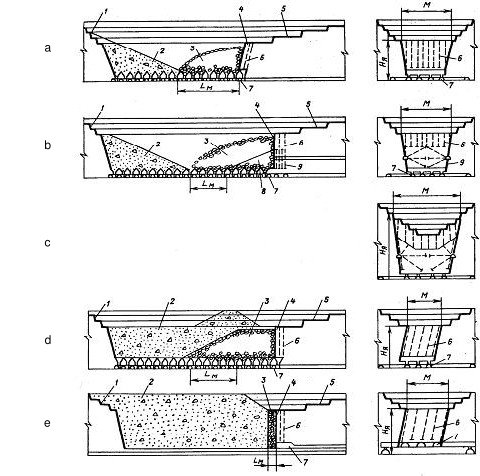
\includegraphics[width=0.8\textwidth]{image74}
    \caption*{a - without loading the sides and ledge with rock mass; b - with
partial loading of the ledge with broken rock; c - with the completion
of deep horizons in an open way without additional separation of the
sides of the quarry; d, е - with full loading of the ledge and sides of
the worked space, respectively, with bottom and end ore release; 1 -
non-working side of the quarry; 2 - internal dump; 3 - ore mass; 4 -
ledge of the open-underground tier; 5 - working side of the quarry; 6
- parallel descending wells; 7 - output workings;
8 - loading of the ledge; 9 - fan wells}
    \caption*{Figure 1 - Principal variants of an integrated open-underground method development}
\end{figure}

\begin{multicols}{2}
With an increase in the height of the open-underground tier and a
decrease in the width of the upper working area, the zone of
concentration of compressive stresses expands, and the stresses
themselves increase, at the same time, the zone of tensile stresses is
removed from the ledge. Drilling and exhaust workings outside the lower
part of the ledge and loading a high ledge with a collapsing rock mass
can reduce the concentration of stresses in the selected zones.

On the basis of the bulk medium model, an analysis of the stability of
the vertical ledge was carried out {[}5-6{]}. It has been established
that the stability of an undisturbed vertical ledge composed of
quartzites is ensured when the beaten ore is loaded, located at the
angle of the natural slope of its entire surface, with the exception of
the upper part, at a height equal to the depth of the vertical crack of
separation. Studies carried out by the laboratory of Rock Pressure
Problems of the IPKON RAN on the example of the Annovsky deposit have
shown that the loading of a high ledge ensures its stability even in the
presence of unfavorably oriented cracks in the array. In contrast to the
periodically (once every 1-2 months) collapsed ledge, the stability of
the sides of the developed space must be ensured during the entire life
of the transition zone.

The study of stress fields in the sides of the open-underground tier for
the conditions of the Annovsky deposit was carried out using the
polarization-optical method. It is established that at the height of the
tier 100-120 m, the stability of the unloaded sides of the developed
space is achieved at their slope angle of no more than 70°. The
dependence of the safe slope angles of the ab sides (degree) on the
height of the open-underground tier, taking into account the strength of
the K\textsubscript{k} rocks, can be represented as

\[a_{\delta} = \text{arcctgK}_{k} \cdot H_{\text{я}},(1)\]

The flattening of the sides of the worked-out space as the depth of the
worked-out space increases leads to the fact that the width of its
bottom gradually decreases. At the maximum height of the tier, the
section of the developed space takes the shape of a triangle (Figure 2).
This height Н\textsubscript{maх} (m) depends on the thickness of the
deposit M

\[H_{\text{max}} = \sqrt{\frac{M}{2K_{k}}},(2)\]
\end{multicols}

\begin{figure}[H]
    \centering
    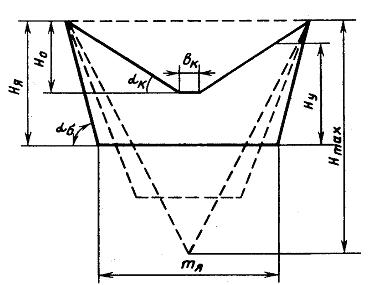
\includegraphics[width=0.8\textwidth]{image75}
    \caption*{Figure 2 - Change in the cross-section of the developed space with
options involving the flattening of its sides with an increase in the
height of the tier}
\end{figure}

\begin{multicols}{2}
Н\textsubscript{y} - the height of the open-underground tier;
Н\textsubscript{o} - the depth of the completion of reserves in an open
way without spreading the sides of the quarry; α\textsubscript{к} - the
angle of the slope of the sides of the quarry during completion;
В\textsubscript{к} - the width of the bottom of the quarry;
α\textsubscript{b} - the angle of the slope of the sides of the
worked-out space of the open-underground tier; m\textsubscript{я} - the
width of the bottom of the worked-out space; Н\textsubscript{maх} - the
maximum possible height of the open-underground tier

The maximum cross-sectional area of the developed space and,
accordingly, the largest volume of reserves in the open-underground tier
corresponds to its height equal to 0.8 H\textsubscript{max}.

The necessary stability of the developed space in the period between the
end of ore release and the beginning of internal dumping is provided by
the choice of a safe angle of slope of the sides, which requires the
abandonment of ore triangles; their volume increases with the height of
the open-underground tier and the decrease in the angle of incidence of
the ore body.

Reduction of ore losses in triangles can be achieved by constant and
complete loading of the sides of the worked-out space with rock mass.
The possibilities of controlling the stability of the array in this case
were considered using numerical modeling of its stress-strain state by
the finite element method on the example of the Tarynnakh iron ore
deposit. It is established that the factors that have the greatest
impact on the stability of the hanging side are the height of the
open-underground tier and the angle of incidence of the ore body.
Stability is maintained at an angle from 60 to 90° and a tier height of
about 80-100 m. At the same time, the zones of possible local
destruction and cracking are located in the lower part of the side of
the quarry from the hanging side and in its upper part from the
recumbent side. However, the presence of such zones does not violate the
stability of the system as a whole.

{\bfseries Results and discussion.} The results of the assessment of the
geomechanical state of the massif made it possible to form three main
options for complex open-underground mining, differing in the way of
ensuring the stability of the ledge and the sides of the developed
space.

The first option provides for the complete release of ore after each
cycle of stripping, leaving only a small ore cushion (Figure 3, a). The
stability of the ledge and the sides of the worked-out space, which are
in an unloaded state for a certain time, is ensured by giving them safe
slope angles. The inner dump is formed with a lag from the ledge without
contact of the waste rock with the ore mass. At the same time, free
bottom release of ore is carried out over the entire area occupied by
the recaptured ore. This option, according to geomechanical conditions,
ensures the creation of an open-underground tier with a maximum height
of 80-100 m using quarry machines for drilling with the formation of
only a lower cut without an underground drilling horizon. It is
advisable to use it at a deposit capacity of no more than 130-150 m,
when the height of the tier will be at least 0.8 H\textsubscript{max}.

In the second variant, after each breakout cycle, a part of the beaten
ore is stored in contact with the ledge, and the internal rock dump is
formed similarly to the first variant. In this case, the stability of
the ledge of the open-underground tier is ensured by priming it with
beaten ore, and the stability of the sides of the worked-out space is
provided by giving them a safe angle of slope.

The full release of ore is carried out only outside the loading, within
the boundaries of which only 10-15\% of the volumes are extracted to
create the necessary loosening. Depending on the size of the loading,
the height of the ledge under geomechanical conditions can be increased
to 150-170 m, which makes it necessary to form an underground drilling
horizon above the bottom level outside the stress concentration zone and
conduct exhaust workings under the bulk of the beaten ore. This option
provides the maximum cross-sectional area of the developed space with a
deposit capacity of up to 200-250 m. With higher power, modifications
can be used that provide for the completion of the upper part of the
open-underground tier reserves in an open way without additional side
spacing (Figure 3, c).
\end{multicols}

\begin{figure}[H]
    \centering
    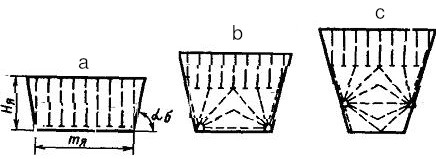
\includegraphics[width=0.8\textwidth]{image76}
    \caption*{Figure 3 - Schematic diagrams of the opening of the ledge of the
open-underground tier}
\end{figure}

\begin{multicols}{2}
The conditions of free ore release characteristic of the considered
options allow increasing the distance between the bottom outlet workings
to 15-20 m, which ensures an increase in reserves per outlet to 150-200
thousand tons.

The third option involves the constant filling of the entire worked-out
space with rock mass. This is due to the need to break off the entire
ledge on the clamping medium and makes it possible to use both an area
and an end outlet (Figure 1 d, e). The height of the tier is limited to
70-90 m both according to the conditions of stability of the hanging
side, and based on the possibilities of rebounding in a clamped
environment. In case of areal release, after each breakout cycle, an
internal dump is built up with the placement of rock above the ore mass;
ore release is carried out at some distance from the ledge where the
dump has reached the design height. At the end outlet, after each
breakout cycle, a complete extraction of the ore mass is carried out
with vertical contact with the rocks of the inner dump. The use of
options with constant filling of the entire worked-out space with rock
mass is advisable when the deposit capacity is up to 80-100 m.

The effectiveness of complex open-underground mining largely depends on
the reasonable choice of parameters and indicators of drilling and
blasting operations.

In principle, three main schemes for the construction of a high ledge
are possible (Figure 4). The first scheme (Figure 3, a) provides for
drilling the entire ledge with parallel descending wells using quarry
machines. This makes it possible to abandon the creation of an
underground drilling horizon, but requires the formation of a lower cut.
Based on the characteristics of the most powerful quarry equipment, the
height of the tier in this case does not exceed 70-90 m, taking into
account the cutting.

The second scheme (Figure 3, b) assumes the formation of an underground
drilling horizon at the level of the release horizon and the rebounding
of the lower part of the ledge with fan wells. The maximum height of the
tier in this case can reach 120-140 m.

The disadvantages of the location of drilling workings in the stress
concentration zone make the third scheme more promising (Figure 3, c),
which provides for drilling horizon above the bottom level and drilling
of the lower part of the ledge with ascending and descending fan wells.
In this case, the parameters of the existing drilling equipment allow
increasing the height of the tier to 160-170 m.

The main feature of the rebound in open-underground mining is the
significant depth of blast wells, with the growth of which their
deviation from the design position increases. As a result, the
consumption of explosives in certain parts of the exploding array
becomes less than the calculated one, which leads to a deterioration in
the quality of crushing.

Based on data on well deviations at a number of domestic and foreign
enterprises and taking into account experience in reducing these
deviations, the dependences of the oversized yield on the height of the
open-underground tier were calculated and it was found that with the
appropriate parameters of drilling and blasting operations and a
conditioned piece of 1000 mm, the oversized yield should not exceed
10\%. The effective release of ore of such a granulometric composition
with significant reserves per outlet can be ensured through the use of
high-unit power technical means, which include heavy vibratory feeders,
loading and delivery machines with a large bucket capacity and hydraulic
excavators. This equipment should work in combination with the most
productive transport equipment.

The technical and economic analysis showed that in the variants with
free ore release, it is advisable to use a complex vibrating feeder of
the RPU type - rail transport using heavy-duty wagons with a load
capacity of 20 tons or more. With options with constant filling of the
worked-out space and release under the overlying rocks with the use of
area release, the most promising is the use of powerful loading and
transport machines with ore delivery to the ore outlet. Excavators in
combination with underground dump trucks or trolleybuses can also be
used for the end release.

Studies were devoted to the problem of the organization of ventilation
of mine workings with a complex open-underground method, as a result of
which, based on the study of the mode of air movement during filtration
through the collapse zone, the use of a combined suction-discharge
ventilation scheme was recommended, which allows a wide range of
operating modes of suction and discharge fans.

An indicator of the intensity of field exploitation within the
open-underground tier is the rate of movement of a high ledge, which, in
combination with the cross-sectional area of the developed space,
determines the possible production volumes. The speed of moving the
ledge, in turn, depends on four main factors: the rate of advance of the
front of work in the quarry, the intensity of drilling and blasting, the
release and transportation of ore and internal dumping.

The rate of movement of the operational front under the condition of
drilling and blasting operations and ore release
v\textsubscript{f}\textsuperscript{b.v} (m /year) is determined based on
the maximum number of relevant equipment in simultaneous operation of
the pob, and its unit productivity Q\textsubscript{ob}, depending on the
adopted technology and the parameters of the tier

\[v_{\text{ф}}^{\text{б.в}} = \frac{n_{\text{об}} \cdot Q_{\text{об}} \cdot N_{\text{см}} \cdot N_{\text{год}}}{S_{\text{в}} \cdot \gamma_{\text{р}}},(3)\]

where Q\textsubscript{ob} is the shift productivity of a unit of
equipment, t/shift; N\textsubscript{cm} is the number of working shifts
per day; N\textsubscript{год} is the number of working days per year;
S\textsubscript{в} is the cross-sectional area of the worked space,
m\textsuperscript{2}; γ\textsubscript{р} is the average ore density,
t/m\textsuperscript{3}.

The rate of advance of the front according to the condition of internal
dumping v\textsubscript{f} (m/ year) is

\[v_{\text{ф}}^{\text{отв}} = \frac{n_{\text{об}^{0}} \cdot Q_{\text{об}^{0}} \cdot N_{\text{см}} \cdot N_{\text{год}} \cdot K_{\text{р}}}{(S_{\text{в}} + S_{\text{k}}) \cdot \gamma_{\text{п}}},(4)\]

Calculations have shown that ensuring the required intensity of
development is achieved mainly due to the development of the ore release
zone.

The variants of the complex open-underground mining method differ in the
level of the upper boundary of the open-underground tier and its height
and are characterized by different volumes of reserves intended for
open, open-underground and underground mining.

With free ore release, the maximum height of the open-underground tier
is determined by the safe slope angles of the sides with a deposit
capacity of up to 150-180 m. With a higher capacity, the height of the
open-underground tier is determined by technological factors, in
particular, the capabilities of drilling equipment. With constant
filling of the worked-out space with rock mass, the maximum height of
the tier is limited by the conditions of breaking in a clamped
environment within 70-90 m.

It has been established that at the new deposit, it is advisable to
place the upper boundary of the open-underground tier at the level of
the maximum depth of the quarry, justified by known methods without
taking into account the features of open-underground mining. In the
conditions of an exploited field, with overburden lagging and increased
requirements for environmental protection, it is advisable to place the
open-underground tier partially within the reserves located in the
contours of the quarry, with a decrease in the maximum depth of the
latter.

Technological options with constant filling of the worked-out space with
rock mass and the release of ore under the overlying rocks of the
internal dump ensure the greatest efficiency of field development at the
maximum permissible height of the open-underground tier located below
the limit of open work.

{\bfseries Conclusion.} Thus, the conducted research and design studies
have established that an integrated open-underground method of
developing strong ores is a promising direction for the development of
subsurface resources. In the appropriate mining-geological and mining
engineering conditions, it allows:

- to reduce the area of environmental disturbance by reducing the volume
of external dumping;

- to significantly compensate for the decrease in ore production volumes
during the development of deep horizons of quarries;

- to reduce the total volume of overburden in the contour of the quarry
due to the development of deep horizons with one high ledge without
additional separation of the sides;

- use general schemes for opening deep horizons of a quarry and
underground mines.

Combined geotechnology makes it possible to identify the main directions
of the implementation of the idea of integrated development of the
subsoil in the field of open-underground mining. These include: a
combination of technological elements of open and underground mining
operations at the stage of treatment excavation, the joint use of open
and underground mining operations for ore transportation, the use of a
single developed space of open and underground mining operations to
accommodate overburden. With a complex open-underground method, all
three of these directions are implemented, but they can also develop
independently in a wider range of mining and geological conditions.
Therefore, an important task of further research should be considered
the development of new technological solutions and the substantiation of
the principles of their design within the framework of the considered
promising areas.
\end{multicols}

\begin{center}
{\bfseries References}
\end{center}

\begin{enumerate}
\item
Puchkov L.A., Sharovar I.I., Vitkalov V.G. Geotekhnologicheskie
sposoby razrabotki mestorozhdenii. - M: Izd-vo ``Gornaya kniga'',
2006. - s. 322.

\item
Lazchenko K.N., Terentyev B.D. Geotekhnologicheskie sposoby
razrabotki mestorozhdenii poleznykh iskopaemykh. - M: MGGU, 2000. - s.
75.

\item
Demidov YU.V. O klassifikatsii sistem kombinirovannoi razrabotki
rudnykh mestorozhdenii // Gornyi zhurnal. - №4, 1995. - s. 16-19.

\item
Kazikaev D.M. Kombinirovannaya razrabotka rudnykh mestorozhdenii. -
M: Izd-vo «Gornaya kniga». - 2008. - s. 355.

\item
Kaplunov D.R., Kalmykov V.N., Rylnikova M.V. Kombinirovannaya
geotekhnologiya. - M: Izd-vo «Ruda i metally». - 2003. - s. 550.

\item
Kaplunov D.R., Rylnikova M.V. Kombinirovannaya razrabotka rudnyh
mestorozhdenij. - M.: Gornaya kniga, 2012. - 344 s.
\end{enumerate}

\begin{center}
\emph{{\bfseries Information about the authors}}
\end{center}

\begin{itemize}
\item
Baizbayev M.B. - Kazakh University of Technology and Business, Astana,
Kazakhstan, \href{mailto:baiz76@mail.ru}{\nolinkurl{baiz76@mail.ru}};

\item
Aliyev S.B. - Institute of Problems of Complex Development of Subsoil
named after academic N.V.Melnikov (IPKON RAN), Moscow, Russian
Federation, \href{mailto:baiz76@mail.ru}{alsamat@yandex.ru};

\item
Shontayev A. D. - Kazakh University of Technology and Business, Astana,
Kazakhstan,
\href{mailto:shon_oskar@mail.ru}{\nolinkurl{shon\_oskar@mail.ru}};

\item
Meiram D. D. - Kazakh University of Technology and Business, Astana,
Kazakhstan,
\href{mailto:diana_meiram@mail.ru}{\nolinkurl{diana\_meiram@mail.ru}};

\item
Karzhauova E. K. - Kazakh University of Technology and Business, Astana,
Kazakhstan,
\href{mailto:karzhauova.81@mail.ru}{\nolinkurl{karzhauova.81@mail.ru}}
\end{itemize}

\begin{center}
\emph{{\bfseries Сведения об авторах}}
\end{center}

\begin{itemize}
\item
Баизбаев М.Б. - Казахский университет технологии и бизнеса, Астана,
Казахстан, \href{mailto:baiz76@mail.ru}{\nolinkurl{baiz76@mail.ru}}:

\item
Алиев С.Б. - Институт проблем комплексного освоения недр имени акад.
Н.В.Мельникова Российской академии наук (ИПКОН РАН), Москва, Российская
Федерация, \href{mailto:baiz76@mail.ru}{alsamat@yandex.ru};

\item
Шонтаев А.Д. - Казахский университет технологии и бизнеса, Астана,
Казахстан,
\href{mailto:shon_oskar@mail.ru}{\nolinkurl{shon\_oskar@mail.ru}};

\item
Мейрам Д.Д. - Казахский университет технологии и бизнеса, Астана,
Казахстан,
\href{mailto:diana_meiram@mail.ru}{\nolinkurl{diana\_meiram@mail.ru}};

\item
Каржауова Э.К. - Казахский университет технологии и бизнеса, Астана,
Казахстан,
\href{mailto:karzhauova.81@mail.ru}{\nolinkurl{karzhauova.81@mail.ru}}
\end{itemize}
